\section{Stars Matching}\label{sec:filter_on_data_graph}
This section describes how we filter on the data graph efficiently by analyzing the user provided searching constraint,
decomposing the pattern graph into stars, and scanning the data graph sequentially.
\subsection{Constraint Analysis}\label{sec:constraint_analysis}
The WHERE clause of a graph matching query specified a constraint or searching condition on the matching results.
The constraint are expressed in the form of predicates, e.g., $=$, $\neq$, $>$, $\ge$, $<$, $\le$.
And the Boolean operator AND ($\land$), OR ($\lor$), NOT ($\lnot$) can be used to combine multiple predicates into a new one.
For example, in Figure~\ref{img:cypher_query}, there are three predicates concatenated by AND\@.
Formally, the constraint is a function $\psi: PG \rightarrow B$ with $PG$ the set of pattern graph and $B$ the set of Boolean values.
We will also use $\psi$ to denote abstract predicate for simplicity in this section:
$\psi(u)$ defines a constraint $\psi$ on vertex $u$, e.g., ``\mintinline{cypher}{id(u4) >= 2020}'' defines a vertex constraint on $u_4$ where the ID of the matching vertex of $u_4$ must great than or equal to $2020$;
and $\psi(u_1, u_2)$ defines a constraint on vertex $u_1$ and vertex $u_2$,
e.g., ``\mintinline{cypher}{id(u1) < id(u2)}'' defines a constraint on $u_1$ and $u_2$ that the ID of the matching of $u_1$ must be less than that of $u_2$.

\textbf{Previous work usually ignore the constraint specification part of a graph matching query.}
If someone wants to query a pattern with a specific searching condition,
she or he has to match the pattern graph first and then filter on the matching results,
which leaves a lot of room for improvement because the user provided searching conditions could filter out many unnecessary
partial results in an early phase.

However, it is still challenging to make use of the constraint provided by user's WHERE clause.
The pattern graph and the constraint are logically two different things,
we have to obtain enough information in order to use the constraint as early filter during the graph matching phase.
For example, the constraint in Figure~\ref{img:cypher_query} include all the vertices in the pattern graph,
\textbf{only when the pattern graph is already matched could we got enough information to apply the constraint},
which makes the constraint filter nearly useless.

\begin{figure}[ht]
  \centering
  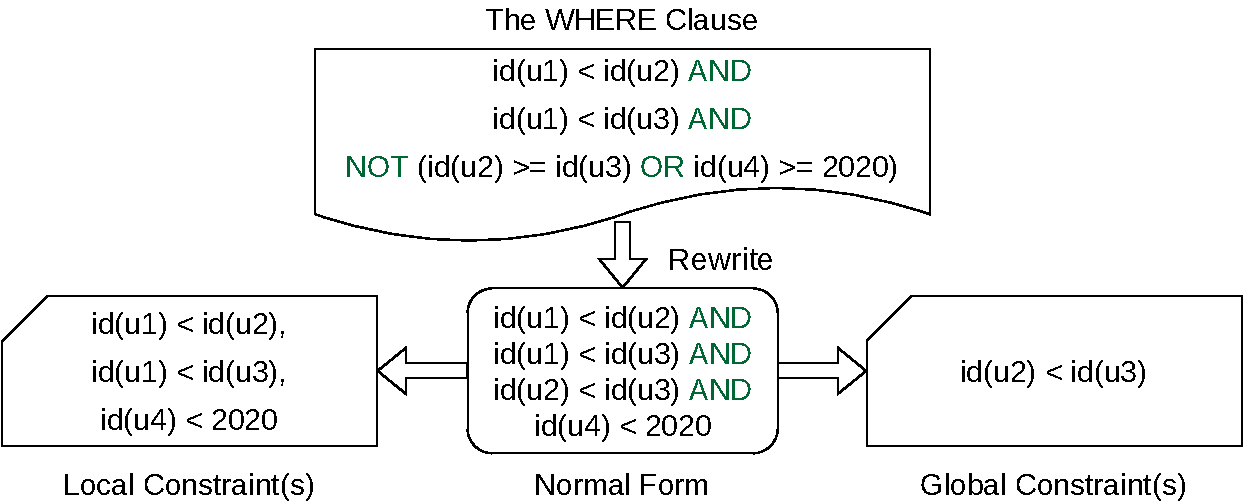
\includegraphics[width=.45\textwidth]{img/constraints.pdf}
  \caption{Constraint Analysis.}\label{img:constraints}
\end{figure}

To address this problem, as shown in Figure~\ref{img:constraints},
we dive into the syntax tree of the graph matching query and decompose the searching condition into smaller parts which require only what we could got during the graph matching phase.
Specifically, we decompose the searching condition into three parts: \emph{vertex constraints}, \emph{edge constraints} and \emph{global constraint}.
A vertex constraint is a function $\psi(u)$ mapping vertex $u$ to Boolean values,
and an edge constraint sets a constraint on edge $(u_1, u_2)$ by a function $\psi(u_1, u_2)$.
For example, in Figure~\ref{img:pattern} ``\mintinline{cypher}{id(u4) < 2020}'' sets a vertex constraint on $u_4$,
``\mintinline{cypher}{id(u1) < id(u2)}'' and ``\mintinline{cypher}{id(u1) < id(u3)}'' are edge constraints,
while ``\mintinline{cypher}{id(u2) < id(u3)}'' is not because there is no edge between $u_2$ and $u_3$.
\textbf{The \emph{vertex constraints} and \emph{edge constraints} are \emph{local constraints} that only require local information that can be obtained during the graph matching phase.
So they could then be pushed down to the data graph scanning phase to short-circuit useless matching results.}
A global constraint $\psi(u_1, u_2, \dots)$ sets a constraint on a series of vertices $u_1, u_2, \dots$,
the information is insufficient during the data graph scanning phase,
however, it still contains many useful information that can be used during the join phase,
and we will discuss it later in Section~\ref{sec:join_on_compressed_data}.

\begin{algorithm}[ht]
  \caption{Constraint Rewriting}\label{alg:rewrite}
  \SetKwFunction{ConstraintRewrite}{\textsc{ConstraintRewrite}}
  \SetKwFunction{Simplify}{\textsc{Simplify}}
  \Input{$expr$: the abstract syntax tree of the WHERE clause}
  \Output{A set of simplified constraints connected by the AND ($\land$) operator}
  \Fn{\ConstraintRewrite{$expr$}}{
    \Match{$expr$}{
      \Case{$\lnot \lnot e$}{\Return{\ConstraintRewrite{$e$}}}
      \Case{$\lnot (e_1 \lor e_2)$}{
        \Return{\ConstraintRewrite{$\lnot e_1$} $\cup$ \ConstraintRewrite{$\lnot e_2$}}
      }
      \Case{$e_1 \land e_2$}{\Return{\ConstraintRewrite{$e_1$} $\cup$ \ConstraintRewrite{$e_2$}}}
      \Case{$e$}{\Return{$\{$ \Simplify{$e$} $\}$}}
    }
  }
\end{algorithm}

Logically, the AND ($\land$) operator create a new constraint $\psi = \psi_1 \land \psi_2$ by combining two constraints $\psi_1$ and $\psi_2$,
where $\psi_1$ and $\psi_2$ can be used to check the matching results independently because there is no side effects in constraints,
so we could safely split $\psi$ into $\psi_1$ and $\psi_2$.
\textbf{Because local constraints are the earliest constraint filters, we should extract as much as possible.}
In order to make the constraint filters more efficient and extract more local constraints:
Firstly, we optimize the AST by classic methods such as compile-time calculation,
handle special cases such as ``\mintinline{cypher}{WHERE false}''.
Then, we apply Algorithm~\ref{alg:rewrite} to analyze the syntax tree and rewrite it into \emph{normal form},
where a normal form is a list of simplified constraints connected by the AND operator.
In fact, the constraints are mostly specified by binary operators such as ``$\le$'', ``$\ne$'',
hence many constraints are naturally local constraints.
And the De Morgan's law enables us to convert the OR ($\lor$) operator into AND ($\land$):
\begin{equation}
  \lnot (\psi_1 \lor \psi_2) = \lnot \psi_1 \land \lnot \psi_2
\end{equation}
So Algorithm~\ref{alg:rewrite} will always keep the semantics of the original user provided constraint.
For example, the third predicate of the AND operator in Figure~\ref{img:cypher_query} would be rewritten to
\begin{minted}[fontsize=\scriptsize]{cypher}
  id(u2) < id(u3) AND id(u4) < 2020
\end{minted}
by applying De Morgan's law.
And the WHERE clause of Figure~\ref{img:cypher_query} would be rewritten to the normal form:
\begin{minted}[fontsize=\scriptsize]{lisp}
  WHERE id(u1) < id(u2) AND id(u1) < id(u3)
  AND id(u2) < id(u3) AND id(u4) < 2020
\end{minted}

\begin{algorithm}[ht]
  \caption{Constraint Pushdown}\label{alg:push_down}
  \SetKwFunction{ConstraintPushdown}{\textsc{ConstraintPushdown}}
  \SetKwFunction{AddVertexConstraint}{\textsc{AddVertexConstraint}}
  \SetKwFunction{AddEdgeConstraint}{\textsc{AddEdgeConstraint}}
  \SetKwFunction{Edges}{\textsc{Edges}}
  \Input{The normal form of constraints $exprs$ and the user described pattern graph $p$}
  \Output{The vertex constraints and edge constraints are pushed down to $p$ and the global constraints will be returned}
  \Fn{\ConstraintPushdown{$exprs$, $p$}}{
    $globals \leftarrow [\,]$\;
    \ForEach{$expr \in exprs$}{
      \Match{$expr$}{
        \Case{$\psi(u)$}{\AddVertexConstraint{$p$, $\psi(u)$}}
        \Case{$\psi(u_1, u_2)$}{
          \If{$(u_1, u_2) \in$ \Edges{$p$}}{\AddEdgeConstraint{$p$, $u_1$, $u_2$, $\psi(u_1, u_2)$}}
        }
        \Case{$e$}{$globals \leftarrow globals \cup \{e\}$\;}
      }
    }
    \Return{$globals$}
  }
\end{algorithm}

The normal form is then used to extract useful information to be pushed down to the pattern graph as in Algorithm~\ref{alg:push_down}.
For each constraint in the normal form, we check if it is local constraint and then push it down to the corresponding vertex or edge.
For example, we would obtain the pattern graph in Figure~\ref{img:pattern_constraint} after doing constraint analysis for the query in Figure~\ref{img:cypher_query}.
After that, We could then decompose it into stars (Section~\ref{sec:star_decomposition}).
Our framework contains a JIT compiler that is able to emit callable closures based on the AST,
and the local constraints can then be used to serve as early filters in the data graph scanning process to short-circuit unnecessary matchings as soon as possible (Section~\ref{sec:data_graph_scanning}).
\begin{figure}[ht]
  \centering
  \resizebox{.7\columnwidth}{!}{
    \begin{tikzpicture}
      \begin{scope}
        \node (C1) at (-3, 1.75) {$C_1: u_1.id < u_2.id$};
        \node (c2) at (3, 1.75) {$C_2: u_1.id < u_3.id$};
        \node (c4) at (3, -2.5) {$C_3: u_4.year < 2020$};
      \end{scope}
      \begin{scope}[every node/.style={circle,thick,draw}]
        \node[label={[label distance=0.6]90:Person}] (1) at (0, 2.25) {$u_1$};
        \node[label={[label distance=1]180:Person}] (2) at (-2.25, 0) {$u_2$};
        \node[label={[label distance=1]0:Person}] (3) at (2.25, 0) {$u_3$};
        \node[label={[label distance=0.6]270:Media}] (4) at (0, -2.25) {$u_4$};
      \end{scope}
      \begin{scope}[>={Stealth[black]},
          every node/.style={fill=white,circle},
          every edge/.style={draw=black}]
        \path [->] (1) edge[bend left=15] node[rectangle,rotate=45] {FOLLOWS} (2);
        \path [->] (2) edge[bend left=15] node[rectangle,rotate=45] {FOLLOWS} (1);
        \path [->] (1) edge[bend left=15] node[rectangle,rotate=-45] {FOLLOWS} (3);
        \path [->] (3) edge[bend left=15] node[rectangle,rotate=-45] {FOLLOWS} (1);
        \path [->] (1) edge[bend left=15] node[rectangle,rotate=-90] {PUBLISHES} (4);
        \path [->] (1) edge[bend right=15] node[rectangle,rotate=-90] {LIKES} (4);
        \path [->] (2) edge node[rotate=-45] {LIKES} (4);
        \path [->] (3) edge node[rotate=45] {LIKES} (4);
      \end{scope}
    \end{tikzpicture}
  }
  \caption{The pattern graph with local constraints pushed down.}\label{img:pattern_constraint}
\end{figure}
\subsection{Star Decomposition}\label{sec:star_decomposition}
\textbf{To design a join based graph matching algorithm, the first thing is to decide what is the basic join unit.}
The simplest join unit is edge, however, it will result in huge amount of useless intermediate results if we use edge as basic unit.
Some authors may adopt more complex structure such as frequent subgraphs as their basic unit,
however, super-linear indices are inevitable for these algorithms~\cite{DBLP:journals/pvldb/SunWWSL12},
and this problem would be more severe for out-of-core environment.
Based on these observations, \textbf{we make a balance by adopting star as our basic matching unit},
where a star $S_k$ is a complete bipartite graph $K_{1,k}$ with one root and $k$ leaves.
For one thing, stars can be matched sequentially without complex indices in a out-of-core environment,
which we will discuss more details in the next section.
And for another, stars can hold enough information, both structural information of the pattern graph and the additional searching constraints provided by user's WHERE clause, to reduce the size of intermediate results.
In this section, we will show how to keep these information as much as possible by decompose the pattern graph into stars properly.

\begin{algorithm}[ht]
  \caption{Star Decomposition}\label{alg:decompose_stars}
  \SetKwFunction{DecomposeStars}{\textsc{DecomposeStars}}
  \SetKwFunction{Peek}{\textsc{Peek}}
  \SetKwFunction{Star}{\textsc{Star}}
  \SetKwFunction{RemoveVertex}{\textsc{RemoveVertex}}
  \Input{The pattern graph $p$ with vertex/edge constraints pushed down}
  \Output{A sequence of stars with a specific order}
  \Fn{\DecomposeStars{$p$}}{
    $results \leftarrow [\,]$\;
    $p' \leftarrow p$\;
    $candidates \leftarrow \{u | \max_{u \in \text{Vertices}(p)}f(u)\}$\;
    \While{$candidates \neq \emptyset$}{
      $root \leftarrow$ \Peek{$candidates$}\;
      $candidates \leftarrow candidates \setminus \{ root \}$\;
      $candidates \leftarrow candidates \cup \{ leaf \mid leaf \text{ is adjacent to } root \text{ in } p'\}$\;
      \RemoveVertex{$p'$, $root$}\;
      $candidates \leftarrow candidates \setminus \{ u \mid u \in p' \land \deg{u} = 0 \}$\;
      $results \leftarrow results \cup \{$ \Star{$p$, $root$} $\}$\;
    }
    \Return{$results$}
  }
\end{algorithm}

As many authors have stated before,
\textbf{the matching order has a significant impact on the performance of a graph matching query}~\cite{DBLP:journals/pvldb/SunWWSL12,DBLP:conf/sigmod/HanLL13,DBLP:journals/pvldb/LaiQLC15}.
In our framework, matching order is determined by the stars' root order.
We conclude that the root order affects the overall performance in two aspects:
First, different matching orders result in different join operations which have different performance.
Second, the size of the star matching result is determined by the root selection.
Hence, we provide two rules respectively to guide the star decomposition algorithm (Algorithm~\ref{alg:decompose_stars}):
\begin{itemize}[noitemsep]
\item The root should be selected in the leaves of the previous star except for the first star.
\item We prefer to select the vertex $u$ such that $f(u)$ is the maximum among the candidates,
  where $f(u) = \frac{\deg \times nc}{freq}$ is a heuristic function on the degree $\deg$ of $u$,
  number of constraints $nc$ and the frequency $freq$ of vertices with the same label of $u$ in the data graph.
\end{itemize}

The first rule indicates that the roots would form a connected vertex cover of the original pattern graph step by step.
\textbf{By doing so, the join operation will always occurred between two adjacent stars},
and we could use a simple index to boost the join operation (Section~\ref{sec:join_on_compressed_data}).
In contrast, for example, if the two stars are totally separated without any common vertices,
then the join result of these stars would be the Cartesian product of respective star matching results,
where most of the rows in the Cartesian product would be invalid.
The Second rule considers both the information of the pattern graph and the distribution of data graph.
We prefer to select root that contains more structural constraints ($\deg$) and user provided constraints ($nc$),
and prefer root with a low label frequency in the data graph.
\textbf{By doing so the matching result of the star could be as small as possible which reduces the I/O cost and alleviates the burden of the later join operation.}

Previous work STwig~\cite{DBLP:journals/pvldb/SunWWSL12} and TwinTwig~\cite{DBLP:journals/pvldb/LaiQLC15} also use stars as their basic matching units.
However, unlike these previous work which are designed for simple graphs, our stars fully support the real-world property graph model, and most importantly, we will show that the star decomposition algorithm of previous work has a lot of room to be optimized.

\textbf{Both STwig and TwinTwig are designed for undirected simple graph,
which has a limited expressiveness and is not suitable for many real-world applications.}
In contrast, we adopt the property graph model which is widely used in industrial graph databases.
Figure~\ref{img:stars} shows the decomposition results of the patter graph in Figure~\ref{img:pattern},
both vertices and edges are labeled and multiple edges may exist between a leaf and the root vertex.
The vertex constraint $C_4$ and edge constraints $C_1$, $C_2$ are also shown in the graph.

\begin{figure}[ht]
  \centering
  \resizebox{.6\columnwidth}{!}{
    \begin{tikzpicture}
      \begin{scope}[every node/.style={circle,thick,draw}]
        \node[label={[label distance=0.6]90:Person}] (1) at (0, 2.25) {$u_1$};
        \node[label={[label distance=1]180:Person}] (2) at (-2.25, 0) {$u_2$};
        \node[label={[label distance=1]0:Person}] (3) at (2.25, 0) {$u_3$};
        \node[label={[label distance=0.6]270:Media}] (4) at (0, -2.25) {$u_4$};
      \end{scope}
      \begin{scope}[>={Stealth[black]},
          every node/.style={fill=white,circle},
          every edge/.style={draw=black}]
        \path (1) edge (2);
        \path (1) edge (3);
        \path (1) edge (4);
      \end{scope}
    \end{tikzpicture}
  }
  \resizebox{.6\columnwidth}{!}{
    \begin{tikzpicture}
      \begin{scope}[every node/.style={circle,thick,draw}]
        \node[label={[label distance=1]180:Person}] (2) at (-2.25, 0) {$u_2$};
        \node[label={[label distance=1]0:Person}] (3) at (2.25, 0) {$u_3$};
        \node[label={[label distance=0.6]270:Media}] (4) at (0, -2.25) {$u_4$};
      \end{scope}
      \begin{scope}[>={Stealth[black]},
          every node/.style={fill=white,circle},
          every edge/.style={draw=black}]
        \path (2) edge (4);
        \path (3) edge (4);
      \end{scope}
    \end{tikzpicture}
  }
  \caption{The stars generated by previous algorithms.}\label{img:stars_old}
\end{figure}

\textbf{Apart from the graph model differences, we found that existing query decomposition algorithms still have a a lot of room to be improved.}
As we discussed before, the result of the data graph scanning process should be as small as possible to avoid unnecessary I/O cost.
The leaves of a star graph can be viewed as a bunch of constraints on the root vertex,
which help to eliminate useless mappings of the root.
That is to say: \emph{more leaves, more better}.
However, \textbf{previous work ignore the benefits of leaves and leave a lot of room to be optimized}.
Compared to the decomposition result of previous work in Figure~\ref{img:stars},
our algorithm always keeps all the leaves in the pattern graph,
while, the stars of previous work drop many useful leaves.
In some cases, e.g., triangle graph, they even generate stars with only two vertices which reduce to edge decomposition.
Apparently, an edge will result in much more unnecessary matchings than a star.

The key of the optimization of our algorithm is the use of $p'$:
We first copy the pattern graph $p$ and obtain $p'$.
Then we run the vertex cover finding algorithm on $p'$,
vertices are removed one by one in $p'$ while $p$ is always unchanged.
Finally, we use the original $p$ to induce stars.
So the resulting stars will always hold as much leaves as possible,
which improves the performance of data graph scanning significantly.
Experiments show that this simple optimization can reduce the size of matching results to \@???\% of previous work.
\subsection{Data Graph Scanning}\label{sec:data_graph_scanning}
Now, we are ready to elaborate how we match stars efficiently in an out-of-core environment.
First, we will propose our stars matching algorithm by introducing two iterators.
And then we'll show how to implement the two iterators by designing a novel disk format to store the data format,
such that the star matching process is I/O efficient, where \textbf{the huge data graph will be read sequentially without random access, and read at most once}.
\subsection*{Stars Matching}
Random disk access problem is always a challenging problem for out-of-core systems,
especially for the out-of-core graph matching problem where graphs are notorious for their poor locality.
However, in this section, we will show that we could avoid random disk accesses by matching stars using two simple iterators.
Furthermore, our techniques ensure that we would only read the necessary part from the huge data graph file,
and these necessary parts would be only read sequentially once.
That is to say, \textbf{we could match all the stars by scanning only the necessary part of the data graph file sequentially once}.

Consider the first star $star_1$ in Figure~\ref{img:stars}, the root vertex is $u_1$ with the label ``Person'',
and it has three leaves $u_2$, $u_3$ and $u_4$.
To match such a star in a data graph, we should find a star whose root also contains the label ``Person''
and it has at least 3 neighbors that could match $u_2$, $u_3$ and $u_4$ respectively.
Then it is straightforward to obtain an naive method to match $star_1$ in a data graph $d$:
Iterate through \textsc{VertexIter}$(d, Person)$ and check every neighbors of these vertices whether they could match $u_2$, $u_3$ and $u_4$, where \textsc{VertexIter}$(d, l)$ travels through all the vertices with the label $l$ in the data graph $d$.
For example, in Figure~\ref{img:data}, $d[v_1]$, the induced graph of $d$ on $v_1$, is such a star that could match $star_1$.

However, this naive star matching method has a great drawback for vertices with a high degree.
Consider the second star $star_2$ in Figure~\ref{img:stars}, the root vertex is $u_4$ with the label ``Media''.
And we suppose that in Figure~\ref{img:data}, $v_4$ is such a popular media that millions or even billions of persons have left their likes.
The naive method have to visit all the neighbors of $v_4$ but most of them are useless because there is no vertex with label ``Comment'' in $star_2$.
To solve this problem, we introduce the second iterator \textsc{NeighborIter}$(v, l)$,
which visits the neighbors with the label $l$ of a given data vertex $v$.
By iterating through \textsc{NeighborIter}$(v_4, Person)$, we could skip useless neighbors and only load the necessary ones.

\begin{definition}[VertexIter and NeighborIter]
  In a data graph $d$, given a vertex label $l$, \textsc{VertexIter}$(d, l)$ is a iterator that would visit all the vertices with the label $l$ in $d$ sequentially.
  Given a data vertex $v$ and a vertex label $l$, \textsc{NeighborIter}$(v, l)$ is a iterator that would iterate through the neighbors with label $l$ of $v$ sequentially.
\end{definition}

Now we will answer the question: How to match the neighbors with the help of \textsc{NeighborIter}?
Consider $star_1$ in Figure~\ref{img:stars}, it is easy to find the symmetry in this star.
We say that $u_2$ and $u_3$ are equivalent because they have the same vertex label,
their connections to the root are the same, and the edge constraints $C_1$ and $C_2$ are also equivalent
(Remember that an edge constraint is a function, that in this case $u_2$ and $u_3$ are just free variables).
For simplicity, we introduce the definition \textsc{NeighborInfo} as follows:
\begin{definition}[NeighborInfo]
  A \textsc{NeighborInfo} of a neighbor vertex $n$ is a structure that stores:
  \begin{enumerate}[noitemsep]
  \item the label of the neighbor $n$,
  \item the vertex constraint of the neighbor $n$,
  \item the edges between the root vertex $v$ and the neighbor $n$
    (the direction of the edges may be $v \rightarrow n$, $v \leftarrow n$ or $v \text{---} n$ because a user could ignore the direction of some edges in the pattern graph),
  \item and the edge constraints of the edges.
  \end{enumerate}
\end{definition}
In a star graph, \textbf{the leaves with the same \textsc{NeighborInfo} form a equivalence class,
and there is no need to blindly permute all possible mappings for the vertices in the same \textsc{NeighborInfo} equivalence class}.
Suppose that there are $m$ leaves with the same \textsc{NeighborInfo} in a star, for each leaf there are $n$ vertices that could be matched in the data graph.
We have to use $m!n$ rows to store the matching result if we blindly permute the mappings for the leaves.
In contrast, only $n$ rows are required if we match group these leaves together which reduces I/O cost dramatically.
\textbf{So instead of matching each neighbors directly, we group the leaves of the star pattern graph by their \textsc{NeighborInfo} during the static analyzing phase, and then use the \textsc{NeighborInfo} to match equivalent vertices at the same time.}
For each neighbor in the \textsc{NeighborIter}, we check whether it would be matched by,
firstly, checking the local constraints of the neighbor,
and then checking the edges between the root and the neighbor.

\begin{algorithm}[ht]
  \caption{Stars Matching}\label{alg:match_stars}
  \SetKwFunction{MatchStars}{\textsc{MatchStars}}
  \SetKwFunction{VertexIter}{\textsc{VertexIter}}
  \SetKwFunction{NeighborIter}{\textsc{NeighborIter}}
  \SetKwFunction{InitializeResults}{\textsc{InitializeResults}}
  \SetKwFunction{AppendResult}{\textsc{AppendResult}}
  \SetKwFunction{FinalizeResults}{\textsc{FinalizeResults}}
  \SetKwFunction{VertexConstraint}{\textsc{VertexConstraint}}
  \SetKwFunction{DegreeConstraint}{\textsc{DegreeConstraint}}
  \SetKwFunction{MatchNeighbor}{\textsc{MatchNeighbor}}
  \SetKwFunction{MatchNeighborInfo}{\textsc{MatchNeighborInfo}}
  \SetKwFunction{Flatten}{\textsc{Flatten}}
  \SetKwFunction{NeighborInfos}{\textsc{NeighborInfos}}
  \Input{The data graph $d$ and a list of $stars$ with the same root label}
  \Output{A list of compressed star matching $results$ corresponding to the $stars$}
  \Fn{\MatchStars{$d$, $stars$}}{
    $results \leftarrow$ \InitializeResults{$stars$}\;
    \ForEach{$v \in$\VertexIter{$d$, $stars[0].root.vlabel$}}{
      $candidates \leftarrow \{ star | star.root$.\VertexConstraint{$v$} $\land star.root$.\DegreeConstraint{$v$} $\}$\;
      $nlabel\_stars \leftarrow $ groups the $candidates$ by leaves' label\;
      \ForEach{$(nlabel, stars) \in nlabel\_stars$}{
        \ForEach{$n \in$\NeighborIter{$v$, $nlabel$}}{
          \MatchNeighbor{$v$, $n$, stars, results}\;
        }
      }
    }
    \FinalizeResults{$results$}\;
    \Return{$results$}\;
  }

  \Fn{\MatchNeighbor{$v$, $n$, $stars$, $results$}}{
    \ForEach{$star \in stars$}{
      \ForEach{$info \in star$.\NeighborInfos{$n.vlabel$}}{
        \If{\MatchNeighborInfo{$v$, $n$, $info$}}{
          \AppendResult{$results[star]$, $n$}\;
        }
      }
    }
  }
\end{algorithm}

By far, there is only one challenge left: How to scan the huge data graph file only once?
The size of the data graph file is proportional to the number of edges in the data graph.
Existing in-memory algorithms would visit the vertices back and forth to explore the data graph,
naively adopt these algorithms to the out-of-core environment would result in numerous swap in/outs,
which is very time consuming and I/O inefficient.
An algorithm that only scan the data graph file sequentially once is desirable,
and we propose a positive answer by providing Algorithm~\ref{alg:match_stars}.
Consider the stars in Figure~\ref{img:stars}, there are two stars that the labels of the roots are different.
\textsc{VertexIter}$(d, Person)$ and \textsc{VertexIter}$(d, Media)$ would be used to visit the vertices in the data graph $d$.
If the data vertices with the same label are stored together in disk,
then the \textsc{VertexIter} could load only the necessary part from disk and visit the vertices sequentially.
Generally speaking, if there are $n$ stars generate by Algorithm~\ref{alg:decompose_stars},
and the size of the labels of the roots is $m$, we have $m \le n$ since multiple stars may have the same label of root.
\textbf{Then we could use $m$ different \textsc{VertexIter} to scan the data graph file by grouping same-label-of-root stars together,
and every iterator would only load a distinct part of the data graph sequentially}
(There is a special case that some stars may isomorphic,
and there is no need to do duplicate star matching, Section~\ref{sec:equivalence_classes} would discuss it in detail).
\textbf{Macroscopically, only the necessary part of the data graph would be loaded to match a pattern graph,
and these parts would be read sequentially only once with the help of \textsc{VertexIter} and \textsc{NeighborIter}.}
\subsection*{Data Graph Disk Format}
To implement the two iterators efficiently, we design a compact disk format to store the data graph (Figure~\ref{img:data_disk_format}).
The disk format is a little bit like to the conventional adjacency list format,
that is, we store a vertex and it's neighbors together.

Specifically, in order to implement the \textsc{VertexIter} efficiently,
\textbf{we should locate data vertices efficiently given a vertex label and visit these vertices without random disk access}.
So \textbf{we store vertices with same vertex label adjacently, and adopt a simple label-to-\textsc{VertexIter} index to boost the searching}.
The \mintinline{text}{num_bytes} field would be used to calculate the position of the next data vertex,
such that the \textsc{VertexIter} can visit the data vertices on disk sequentially to reduce I/O cost.
Apart from that, we also store in-degree and out-degree which can be used as early filters during the star matching process.

For the \textsc{NeighborIter}, there is one thing to notice that we adopt the property graph model,
all edges are directed and multi-edges may exist between a pair of vertices.
To store these information, a naive method is to store in-edges and out-edges for each data vertex.
However, this naive method will be very inefficient when matching property graphs.
Consider the pattern graph in Figure~\ref{img:pattern},
suppose that in a data graph $v_1$ matches $u_1$ and we want to check whether $v_2$, a neighbor of $v_1$, matches $u_2$,
then we have to scan all the in-edges to find if there is an edge from $v_2$ to $v_1$ with label ``FOLLOWS'',
and all the out-edges to check if there is an edge from $v_1$ to $v_2$ with the same label.
Real-world graphs usually have a high skewness, for example, a celebrity in a social network may have millions of followers.
\textbf{These ``celebrities'' will become bottleneck if we adopt the naive method to scan all the adjacent edges.}
To solve this problem, we propose a novel schema to store the neighbors,
\textbf{all the edges connected to a neighbor are stored together with the neighbor,
so the neighbor can be checked in place without scanning all the in-edges/out-edges of the root vertex}.
And we also use a simple label-to-\textsc{NeighborIter} index to boost the searching of neighbors given the label of neighbor.
The position of the next neighbor could be calulated by the \mintinline{text}{num_n_to_v} and \mintinline{text}{num_v_to_n} fields.
And we could use \textsc{NeighborIter} to travel through the neighbors sequentially without random disk access.

\begin{figure}[ht]
  \centering
  \begin{minted}[fontsize=\tiny]{text}
+-----------------------------------------+
|             num_vlabels: k              |
+-----------------------------------------+
+-------------+-------------+-------------+
|   vlabel    |     pos     |     len     |<-+
+-------------+-------------+-------------+  |
|   vlabel    |     pos     |     len     |  |
+-------------+-------------+-------------+  |- k rows
                    ...                      |
+-------------+-------------+-------------+  |
|   vlabel    |     pos     |     len     |<-+
+-------------+-------------+-------------+
+--------------------+--------------------+
|     num_bytes      |         v          |<-----------------------------+
+--------------------+--------------------+                              |
|      in_deg        |      out_deg       |                              |
+--------------------+--------------------+                              |
|               num_vlabels               |                              |
+-----------------------------------------+                              |
+-------------+-------------+-------------+                              |
|   vlabel    |     pos     |     len     |<-+                           |
+-------------+-------------+-------------+  |                           |
|   vlabel    |     pos     |     len     |  |                           |
+-------------+-------------+-------------+  |- num_vlabels rows         |
                    ...                      |                           |
+-------------+-------------+-------------+  |                           |
|   vlabel    |     pos     |     len     |<-+                           |
+-------------+-------------+-------------+                              |     One
+-----------------------------------------+                              |- VertexNode
|                    n                    |                              |
+--------------------+--------------------+                              |
|    num_n_to_v      |    num_v_to n      |                              |
+--------------------+--------------------+                              |
+-----------------------------------------+                              |
|                 elabel                  |<-+                           |
+-----------------------------------------+  |                           |
|                 elabel                  |  |  num_n_to_v + num_v_to_n  |
+-----------------------------------------+  |-           rows           |
                    ...                      |                           |
+-----------------------------------------+  |                           |
|                 elabel                  |<-+                           |
+-----------------------------------------+                              |
                    ...                    <-----------------------------+

  \end{minted}
  \caption{Data graph disk format. (TODO\@: Update this figure.)}\label{img:data_disk_format}
\end{figure}

The vertices are sorted by their ID in the data graph, which is very helpful for the join operation (Section~\ref{sec:join_on_compressed_data}).
Given a series of vertices and a series of edges with arbitrary order,
the data graph file could be generated in sorting time.
And for simplicity, we ignore the key-value properties of a property graph and focus on the labels.
In fact, these properties can be added to our disk format by simply add the corresponding fields.
And the simplicity of the \textsc{VertexIter} and \textsc{NeighborIter} also makes it possible to implement them on other platform, e.g., industry-tested relational database, which we will study in future work to make dynamic property graph transactions and analysis easier.
